\section{Case Studies}
\label{sec:cases}

\subsection{NIO: the same-JVM double run that reruns cannot see}

Our motivating example, \texttt{enums} in \texttt{junit-quickcheck}
(\texttt{quickcheck485}), is also our cleanest NIO case study; its full
trajectory appears in Figure~\ref{fig:case}. Step 0's three isolated reruns
all pass; the planner reads the test source, hypothesizes that nested
JUnitQuickcheck classes leave static accumulators unreset, and selects T2
(\texttt{runs: 2}). Sub-run 1 \texttt{PASS} and sub-run 2 \texttt{ERROR}
(\emph{expected: $<$100$>$ but was: $<$200$>$}) confirm the accumulation. The
diagnoser commits to NIO (confidence 0.98) and cites the static accumulator
(lines~83--90) and the failing assertion (line~460), both inside the region
the developer later fixed. Total cost: 2 LLM calls, 4 executions, 31 seconds,
\$0.0038 — and no rerun-based baseline can ever succeed on this test.

\subsection{OD: static factory state left behind by a sibling test}
\label{sec:case-od}

\texttt{DirectoryManagerFactoryTest\#createDirectoryManagerIoException} in
\texttt{wikidata-toolkit} (\texttt{wdtk-util}) is our cleanest OD case. The
victim expects \texttt{IOException} from
\texttt{DirectoryManagerFactory.createDirectoryManager("/nonexistent/...", true)}
when the factory is configured with the real
\texttt{DirectoryManagerImpl}, which validates the path and throws. Step 0's
three isolated reruns all pass: in isolation the test always installs the
right manager class. The planner reads the two sibling tests and forms the
hypothesis that the factory's \emph{static} manager class is the shared
state: \texttt{createDirectoryManagerNoConstructor} calls
\texttt{setDirectoryManagerClass(TestDirectoryManager.class)}, and the inner
\texttt{TestDirectoryManager} has no \texttt{(Path, boolean)} constructor, so
a subsequent \texttt{createDirectoryManager} reflection call fails with
\texttt{RuntimeException} instead of reaching the \texttt{IOException} path.
It selects T5 with exactly that polluter; the victim then fails on the first
attempt. The diagnoser commits to OD with confidence 0.98 and grounds the
diagnosis in three evidence sites --- the polluter's mutation of the static
field (lines~111--113), the polluting \texttt{TestDirectoryManager}'s
constructor set (lines~37--83), and the victim's
\texttt{@Test(expected=IOException.class)} assertion (lines~116--119).
The developer's fix confirms the mechanism exactly: a
\texttt{@Before} hook resets the manager class to
\texttt{DirectoryManagerImpl.class} before every test. Two LLM calls, four
executions, 21.5 seconds, \$0.0023. NaiveRerun can never observe this failure
(no single run fails); OrderShuffle would need the one specific polluter to
precede the victim within its randomized order, which the agent instead
targets directly from source evidence.

\subsection{TD: a timing race reproduced by parallel execution, not the injected sleep}
\label{sec:case-td}

\texttt{TestInstallSnapshotNotificationWithGrpc\#testInstallSnapshotNotificationCount}
in \texttt{ratis} (\texttt{RATIS-1363}) shows the loop reaching a TD failure
by a route the dataset's own patch does not. The test boots a
\texttt{MiniRaftCluster} over gRPC and asserts that exactly 20
\texttt{InstallSnapshotNotification} events arrive
(\texttt{assertEquals(expectedNotificationCount, notificationCount.get())},
line~280). Step~0's three isolated reruns all pass. The planner's first
hypotheses target timing and shared state: T7 (CPU/IO stress, two cpus) fails,
T2 (same-JVM double run) fails, and T6 injects a 500\,ms sleep at the entry of
the \emph{test method} — the only method name visible cold-start — which also
fails, because the sensitivity lives in the asynchronous gRPC delivery path in
production code, not in the test body. After a second, heavier stress attempt
(four cpus), the planner switches family to T10 (parallel class execution,
four threads) and the assertion fails: \emph{expected $<$20$>$ but was
$<$19$>$}. The diagnoser commits to TD with confidence 0.6 and cites three
sites in the test class — the cluster bootstrap (line~252), the failing count
assertion (line~280), and the gRPC transport subclass that delivers
notifications on separate threads — matching the mechanism. Notably, the
dataset's own reproduction patch for this test injects
\texttt{Thread.sleep} into \texttt{BaseStateMachine} in \emph{production}
code; the agent instead reproduced the race through a transport-level
perturbation it derived from the failure, without ever seeing that patch.
Six LLM calls, eight executions, 73\,s, \$0.0037.

\begin{figure}[t]
\centering
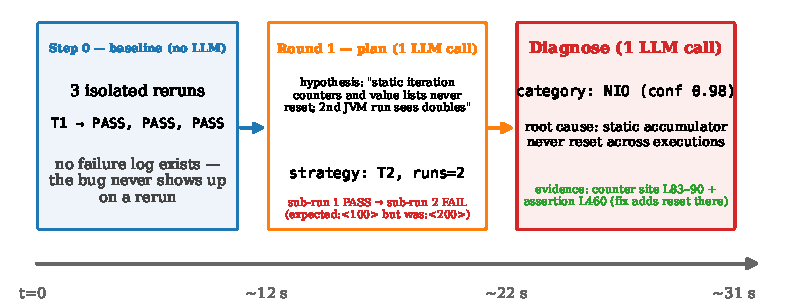
\includegraphics[width=0.9\columnwidth]{figures/case_timeline.pdf}
\caption{Decision timeline of FlakeAgent on the \texttt{enums} NIO case:
each round's hypothesis, strategy, observation, and the final diagnosis with
its evidence.}
\label{fig:case}
\end{figure}
